\chapter{Thiết kế hệ thống}
\section{Kiến trúc tổng thể hệ thống}
Kiến trúc được cung cấp phân tách rõ ràng vai trò giữa Client và Server:
\begin{itemize}
    \item \textbf{Client (Lớp máy khách):} Gồm ứng dụng di động, cổng thông tin cho nhà cung cấp y tế và trang quản trị. Chúng chịu trách nhiệm về giao diện người dùng (UI) và trải nghiệm người dùng (UX).
    \item \textbf{Server (Lớp máy chủ):} Là bộ não của hệ thống, xử lý toàn bộ logic nghiệp vụ, quản lý dữ liệu và giao tiếp với các dịch vụ bên thứ ba.
\end{itemize}
Điểm nổi bật của kiến trúc này là việc áp dụng mô hình \textbf{Microservices}: thay vì xây dựng một ứng dụng máy chủ nguyên khối, hệ thống được chia thành các dịch vụ nhỏ, độc lập (Authentication, Core Healthcare, AI/ML, Notification). Các thành phần như \textbf{API Gateway}, \textbf{Load Balancer}, và \textbf{Message Queue} là những yếu tố then chốt giúp các dịch vụ này hoạt động hiệu quả, có khả năng mở rộng và phục hồi tốt.

\subsection{Lý do Chọn Kiến trúc Client-Server}
Việc lựa chọn kiến trúc Client-Server là hoàn toàn hợp lý và gần như là tiêu chuẩn cho loại ứng dụng này vì những lý do sau:
\begin{itemize}[leftmargin=*]
    \item \textbf{Quản lý dữ liệu tập trung (Centralized Data Management):} Dữ liệu y tế cực kỳ nhạy cảm và cần được quản lý một cách nhất quán, an toàn tại một nơi.
    \item \textbf{Bảo mật và Kiểm soát truy cập (Security \& Access Control):} Cho phép triển khai các cơ chế xác thực và phân quyền (như JWT, RBAC) một cách hiệu quả tại máy chủ.
    \item \textbf{Logic nghiệp vụ phức tạp:} Các quy trình như đặt lịch hẹn, xử lý thanh toán, đưa ra khuyến nghị y tế... đòi hỏi logic phức tạp và cần được xử lý một cách đáng tin cậy trên máy chủ.
    \item \textbf{Khả năng mở rộng và bảo trì (Scalability \& Maintainability):} Máy chủ có thể được mở rộng để phục vụ nhiều người dùng hơn mà không cần thay đổi ứng dụng client.
    \item \textbf{Tích hợp với bên thứ ba:} Việc kết nối với các dịch vụ ngoài được quản lý an toàn và hiệu quả từ phía máy chủ.
\end{itemize}

\subsection{Các Kiến trúc Thay thế và So sánh}

\subsubsection{Kiến trúc Monolithic (Nguyên khối)}
Đây là phương pháp truyền thống, trong đó toàn bộ ứng dụng phía máy chủ được xây dựng như một khối duy nhất.
\begin{itemize}
    \item \textbf{Ưu điểm so với kiến trúc hiện tại:}
    \begin{itemize}
        \item Phát triển ban đầu đơn giản hơn.
        \item Triển khai dễ dàng hơn (ban đầu).
        \item Testing End-to-End đơn giản.
    \end{itemize}
    \item \textbf{Nhược điểm so với kiến trúc hiện tại:}
    \begin{itemize}
        \item Khó mở rộng, phải mở rộng toàn bộ ứng dụng.
        \item Ràng buộc công nghệ.
        \item Khó bảo trì khi ứng dụng lớn dần.
        \item Quá trình triển khai chậm và rủi ro cao.
    \end{itemize}
\end{itemize}

\subsubsection{Kiến trúc Peer-to-Peer (P2P - Mạng ngang hàng)}
Trong mô hình này, không có máy chủ trung tâm. Mọi máy tham gia mạng (peers) đều có vai trò như nhau.
\begin{itemize}
    \item \textbf{Ưu điểm so với kiến trúc hiện tại:}
    \begin{itemize}
        \item Khả năng phục hồi cao, không có điểm lỗi trung tâm.
        \item Khả năng mở rộng tự nhiên.
    \end{itemize}
    \item \textbf{Nhược điểm so với kiến trúc hiện tại:}
    \begin{itemize}
        \item Bảo mật và quyền riêng tư \textbf{KÉM}, không phù hợp cho dữ liệu y tế.
        \item Khó đảm bảo tính nhất quán dữ liệu.
        \item Phức tạp trong việc quản lý và cập nhật.
    \end{itemize}
\end{itemize}

\subsubsection{Kiến trúc Serverless}
Đây là một biến thể của kiến trúc Client-Server, nơi việc quản lý máy chủ được trừu tượng hóa hoàn toàn bởi nhà cung cấp đám mây.
\begin{itemize}
    \item \textbf{Ưu điểm so với kiến trúc hiện tại:}
    \begin{itemize}
        \item Giảm chi phí vận hành, không cần quản lý máy chủ.
        \item Chi phí tối ưu, chỉ trả tiền cho thời gian thực thi.
        \item Tự động mở rộng.
    \end{itemize}
    \item \textbf{Nhược điểm so với kiến trúc hiện tại:}
    \begin{itemize}
        \item Có thể có độ trễ "Cold Starts".
        \item Ràng buộc nhà cung cấp (Vendor Lock-in).
        \item Giới hạn về tài nguyên và thời gian thực thi.
        \item Phức tạp trong việc giám sát và gỡ lỗi.
    \end{itemize}
\end{itemize}
\subsection{Kết luận và Diagram}
Kiến trúc \textbf{Client-Server kết hợp Microservices} là một lựa chọn xuất sắc và theo đúng các tiêu chuẩn thiết kế hệ thống hiện đại. Nó giải quyết được các bài toán cốt lõi của một ứng dụng phức tạp như khả năng mở rộng, tính linh hoạt và khả năng bảo trì trong dài hạn. Mặc dù có độ phức tạp cao hơn, những lợi ích mà nó mang lại hoàn toàn xứng đáng với quy mô và tầm quan trọng của một hệ thống y tế.
\begin{figure}[H]
    % Căn giữa hình ảnh
    \centering
    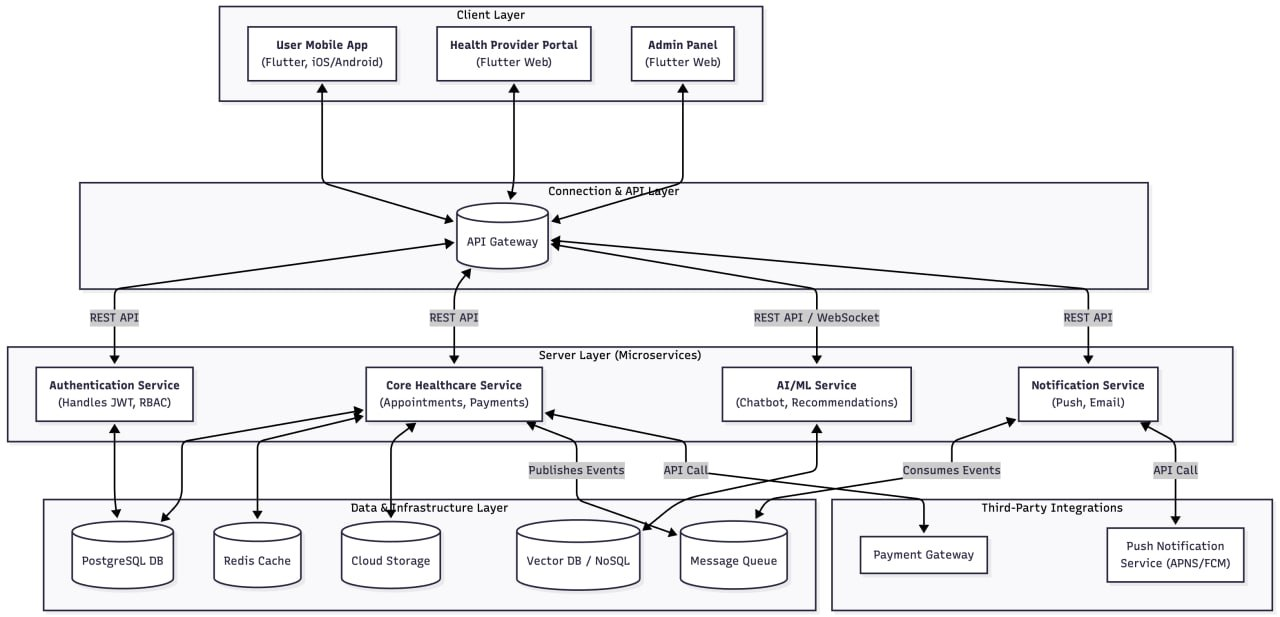
\includegraphics[width=0.8\textwidth]{Images/ArchSys.png}
    \vspace{10pt}
    
    % Thêm chú thích cho hình ảnh
    \caption{Kiến trúc hệ thống}
    
    % Đặt nhãn để tham chiếu chéo (cross-reference)
    \label{fig:sys_arch}
\end{figure}

\section{Thiết kế cơ sở dữ liệu}
\subsection{Mô tả}
Thực thể (ERD) được cung cấp, nhằm mục đích làm rõ cấu trúc dữ liệu và các phân hệ chức năng chính của hệ thống. Mô hình dữ liệu cho thấy đây là một nền tảng công nghệ được thiết kế để kết nối ba nhóm đối tượng chính: Người dùng cuối (Khách hàng), Đối tác cung cấp dịch vụ (Partner), và Nhân viên quản trị (Employee).
\subsection{Các khối chức năng chính}
 Dựa trên các thực thể và mối quan hệ trong sơ đồ, hệ thống được cấu thành từ các khối chức năng (module) chính sau:
 \begin{itemize}
            \item Module Quản lý Tài khoản và Phân quyền (Account Management)
            Đây là module lõi, quản lý định danh và quyền truy cập của toàn bộ người dùng trên hệ thống.
            \begin{itemize}
                \item Thực thể trung tâm: \textbf{Account} lưu trữ thông tin xác thực chung
                \item Cơ chế phân quyền: Hệ thống định nghĩa ba vai trò người dùng riêng biệt với các quyền hạn khác nhau:
                \begin{itemize}
                    \item User: Đối tượng sử dụng dịch vụ.
                    \item Partner: Đối tượng cung cấp dịch vụ/sản phẩm.
                    \item Employee: Đối tượng quản trị và vận hành nền tảng.
                \end{itemize}
                \item Chức năng: Cung cấp cơ chế đăng ký, đăng nhập, xác thực và phân quyền truy cập chức năng tương ứng với từng vai trò.
            \end{itemize}
            \item \textbf{Phân hệ Vận hành dành cho Đối tác (Partner Portal)}: 
            Phân hệ này cung cấp một cổng quản trị toàn diện, cho phép các đối tác số hóa và quản lý hoạt động kinh doanh của mình.
            \begin{itemize}
                \item Quản lý Dịch vụ \& Sản phẩm (Service, Product): Cho phép đối tác khởi tạo, cấu hình giá, mô tả và phân loại các dịch vụ/sản phẩm cung cấp. Thực thể Category giúp hệ thống hóa và hỗ trợ tìm kiếm hiệu quả.
                \item Quản lý Nhân sự (Employee của Partner): Hỗ trợ đối tác quản lý thông tin nhân viên thực hiện dịch vụ.
                \item Quản lý Lịch trình (Schedule): Cung cấp công cụ thiết lập lịch làm việc cho cơ sở và từng nhân viên, làm cơ sở cho tính năng đặt lịch.
            \end{itemize}
        \item \textbf{Phân hệ Trải nghiệm Người dùng (User Experience)} Phân hệ này xây dựng luồng tương tác hoàn chỉnh cho khách hàng cuối.
            \begin{itemize}
                \item Đặt lịch (Booking): Là nghiệp vụ cốt lõi, liên kết các thực thể chính: User, Partner, Service, và Employee (của Partner) tại một thời điểm cụ thể. Trạng thái của lịch hẹn (ví dụ: chờ xác nhận, đã hoàn thành, đã hủy) cũng được quản lý tại đây.
            \item Tìm kiếm và Khám phá: Cấu trúc dữ liệu cho phép người dùng truy vấn, lọc và tìm kiếm dịch vụ/đối tác dựa trên nhiều tiêu chí.
            \item Phản hồi và Đánh giá (Feedback/Review): Sau khi sử dụng dịch vụ, người dùng có thể cung cấp phản hồi, giúp xây dựng độ tin cậy và là cơ sở để đánh giá chất lượng đối tác. 
            \end{itemize}
        \item \textbf{Module Tài chính và Marketing}
        Module này tích hợp các nghiệp vụ liên quan đến giao dịch và các hoạt động thu hút người dùng.
            \begin{itemize}
                \item Xử lý Thanh toán (Payment): Mỗi thực thể Booking được liên kết với một giao dịch Payment, ghi nhận các thông tin về số tiền, phương thức và trạng thái thanh toán.
                \item Quản lý Khuyến mãi (Promotion\(\)Voucher): Cung cấp chức năng tạo và quản lý các chương trình khuyến mãi. Các chương trình này có thể được áp dụng vào giao dịch Booking để điều chỉnh giá trị thanh toán cuối cùng.
            \end{itemize}
        \end{itemize}
\subsection{Kết luận}
Sơ đồ ERD mô tả một cấu trúc dữ liệu chặt chẽ và toàn diện cho một nền tảng dịch vụ đa năng. Từ phân tích trên, có thể xác định các năng lực chính của hệ thống bao gồm:
    \begin{itemize}
        \item Hệ thống quản lý người dùng đa vai trò với cơ chế phân quyền rõ ràng.
        \item Nền tảng đặt lịch (booking platform) thông minh, kết nối nhu cầu của người dùng với khả năng cung ứng của đối tác.
        \item Cổng quản trị dành cho đối tác (partner portal) để tự quản lý vận hành kinh doanh.
        \item Cơ chế thanh toán và khuyến mãi tích hợp, hỗ trợ hoàn chỉnh vòng đời giao dịch và các hoạt động marketing.
        \item Hệ thống thu thập phản hồi và đánh giá, đảm bảo chất lượng và tính minh bạch của nền tảng.
    \end{itemize}
\subsection{Lược đồ}
\begin{figure}[H]
    % Căn giữa hình ảnh
    \centering
    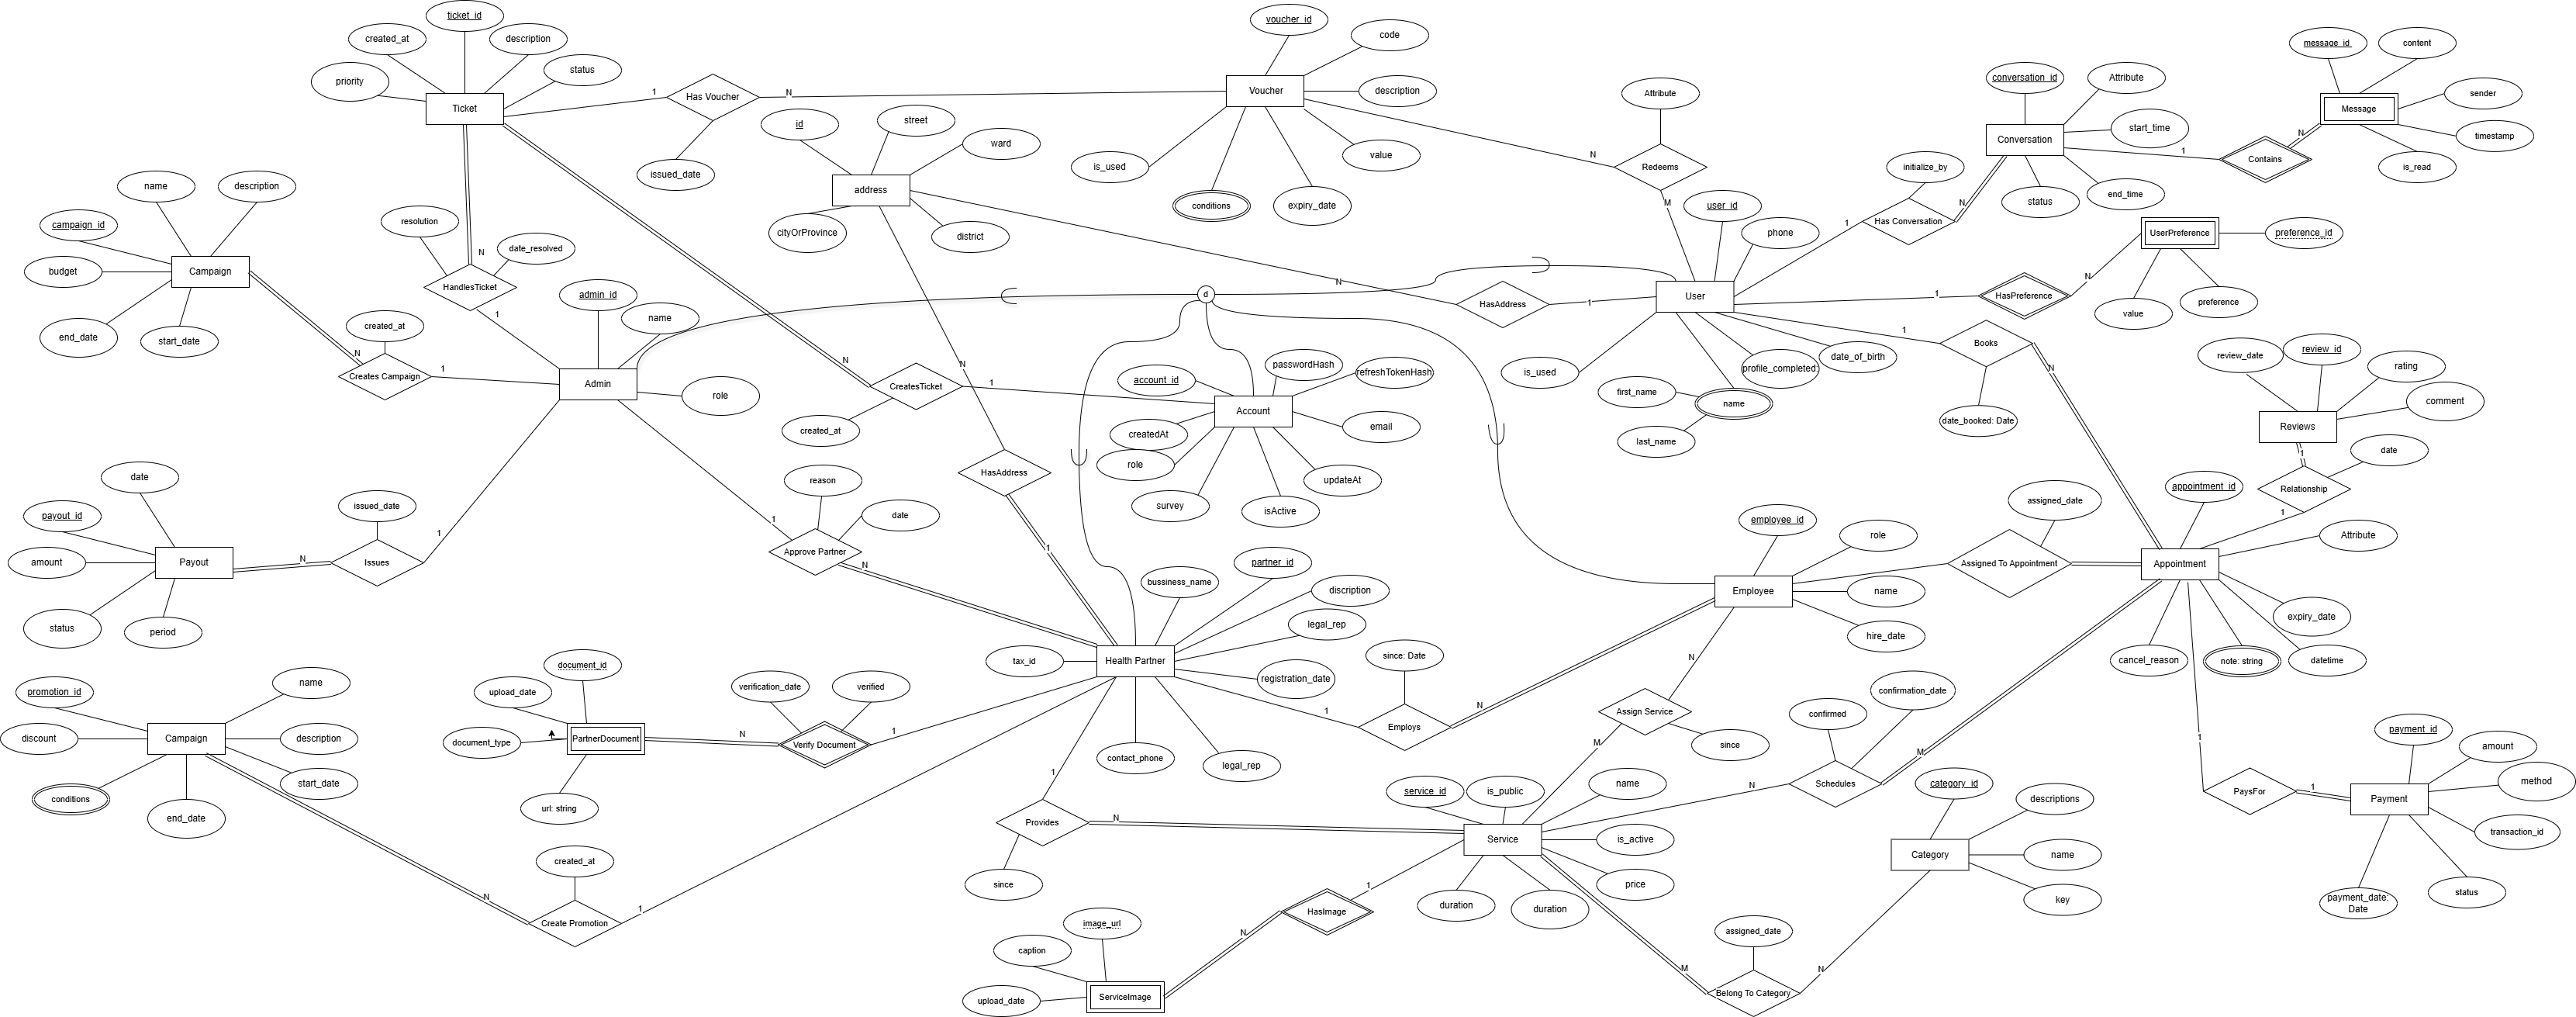
\includegraphics[width=1\textwidth]{Images/ERD.png}
    \vspace{10pt}
    
    % Thêm chú thích cho hình ảnh
    \caption{ER Diagram của hệ thống}
    
    % Đặt nhãn để tham chiếu chéo (cross-reference)
    \label{fig:erd}
\end{figure}


\section{Thiết kế UI/UX cơ bản}
\subsection{Onboarding \& Sign In \& Sign up}
\begin{figure}[H]
    \centering
    
    % --- Hàng 1 ---
    \begin{subfigure}[b]{0.32\textwidth}
        \centering
        % Nếu có ảnh thì dùng dòng dưới:
        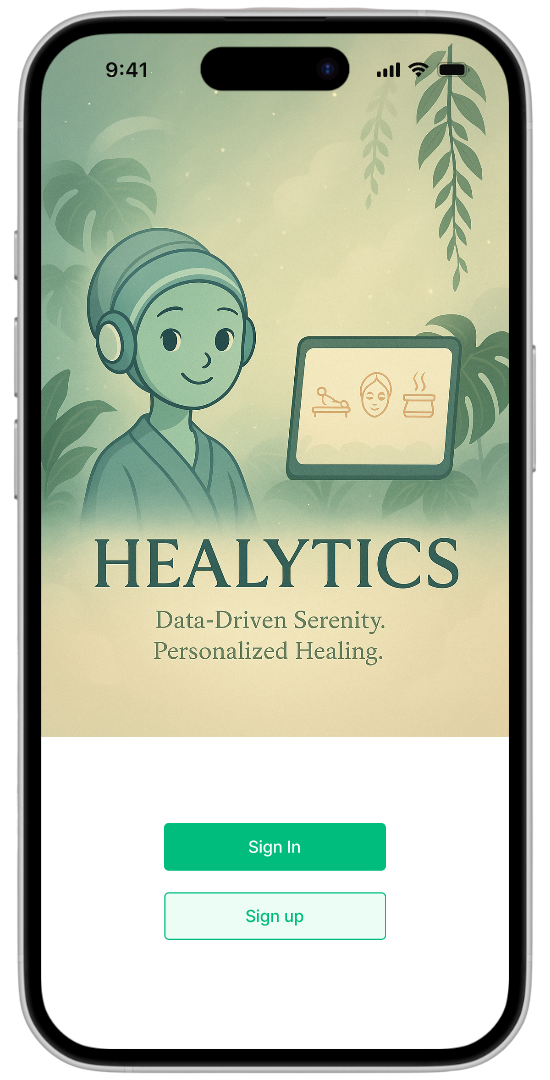
\includegraphics[width=\linewidth]{Images/SignIn_SignUp/onboard.png}
        % Nếu CHƯA có ảnh thì comment dòng trên và mở dòng dưới:
        % \todobox{Splash Screen}
        \caption{Splash Screen}
    \end{subfigure}
    \hfill
    \begin{subfigure}[b]{0.32\textwidth}
        \centering
        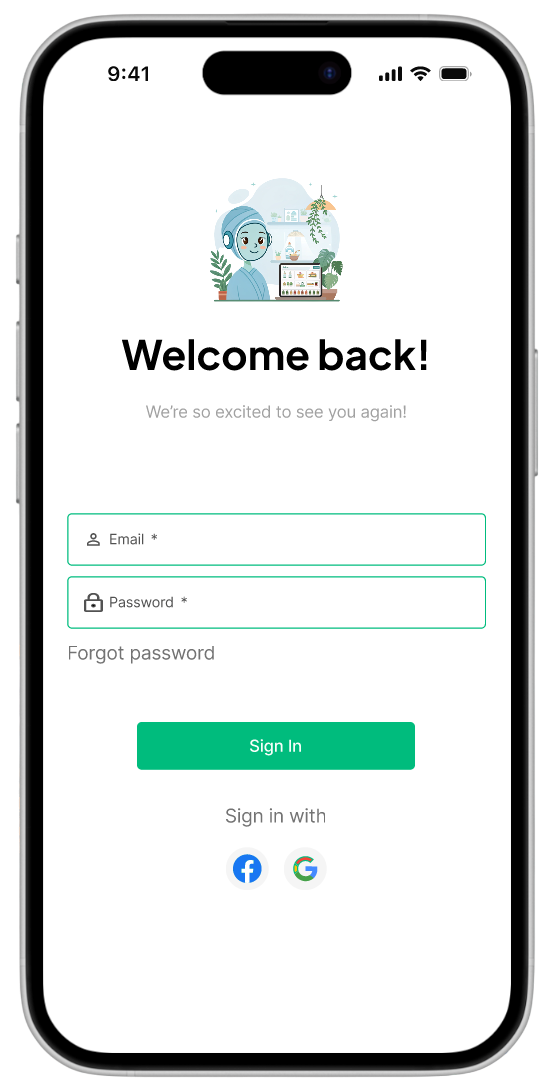
\includegraphics[width=\linewidth]{Images/SignIn_SignUp/signin.png}
        \caption{Login Page}
    \end{subfigure}
    \hfill
    \begin{subfigure}[b]{0.32\textwidth}
        \centering
        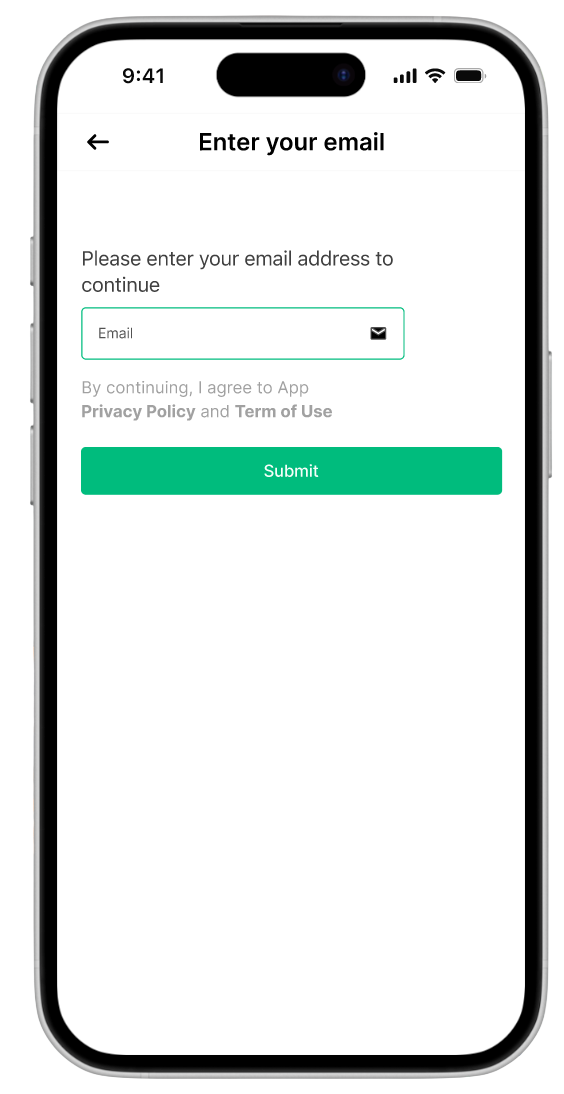
\includegraphics[width=\linewidth]{Images/SignIn_SignUp/signup_email.png}
        \caption{Sign Up}
    \end{subfigure}
    
    \vspace{1em} % Khoảng cách thoáng giữa 2 hàng
    
    % --- Hàng 2 ---
    \begin{subfigure}[b]{0.32\textwidth}
        \centering
        % Lưu ý: Bạn đang dùng lại ảnh signup_email.png, hãy check lại nếu cần
        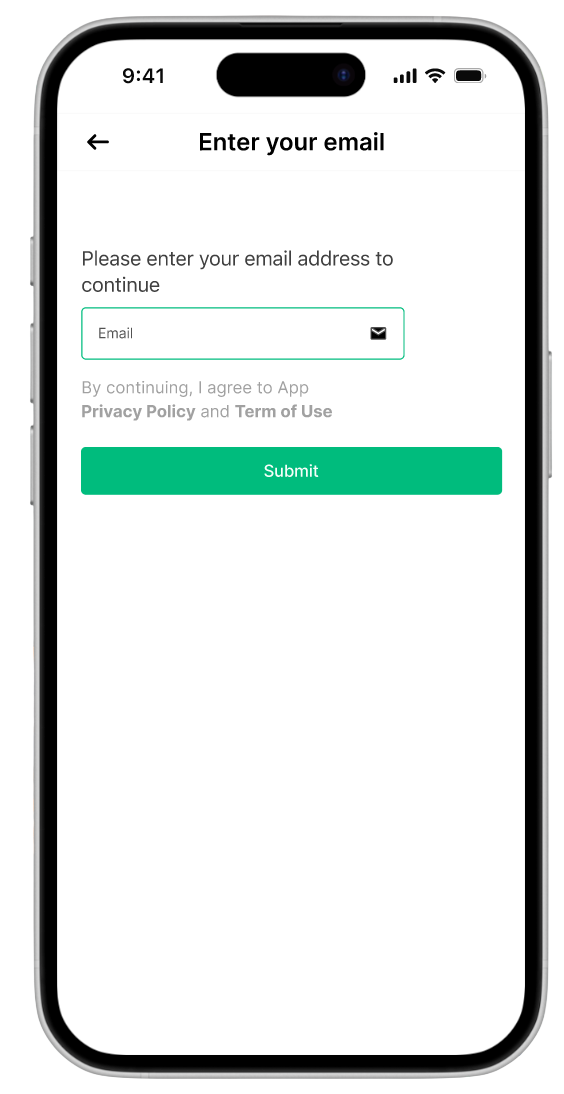
\includegraphics[width=\linewidth]{Images/SignIn_SignUp/signup_email.png}
        \caption{Sign Up Email}
    \end{subfigure}
    \hfill
    \begin{subfigure}[b]{0.32\textwidth}
        \centering
        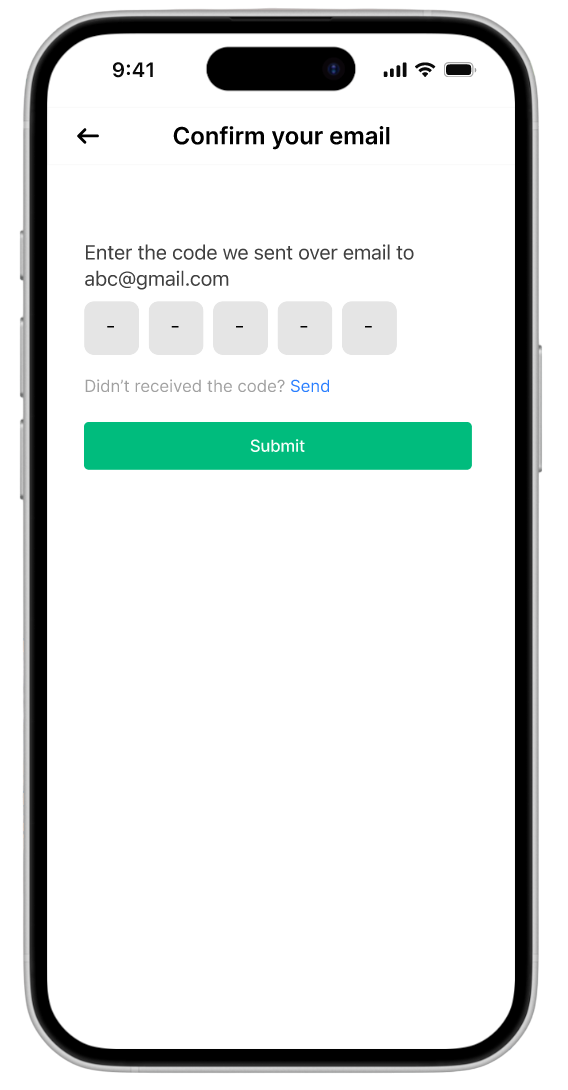
\includegraphics[width=\linewidth]{Images/SignIn_SignUp/signup_otp.png}
        \caption{Sign Up OTP}
    \end{subfigure}
    \hfill
    \begin{subfigure}[b]{0.32\textwidth}
        \centering
         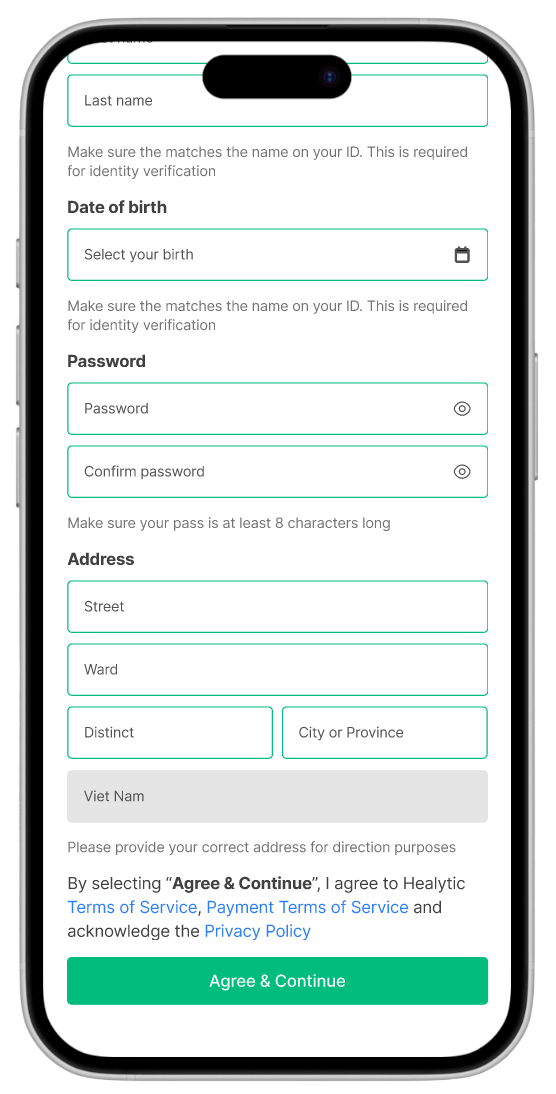
\includegraphics[width=\linewidth]{Images/SignIn_SignUp/signup_finish.png}
        \caption{Sign Up Form}
    \end{subfigure}
\end{figure}
\subsection{Survey}
\begin{figure}[H]
    \centering
    
    % --- Hàng 1 ---
    \begin{subfigure}[b]{0.32\textwidth}
        \centering
        % Nếu có ảnh thì dùng dòng dưới:
        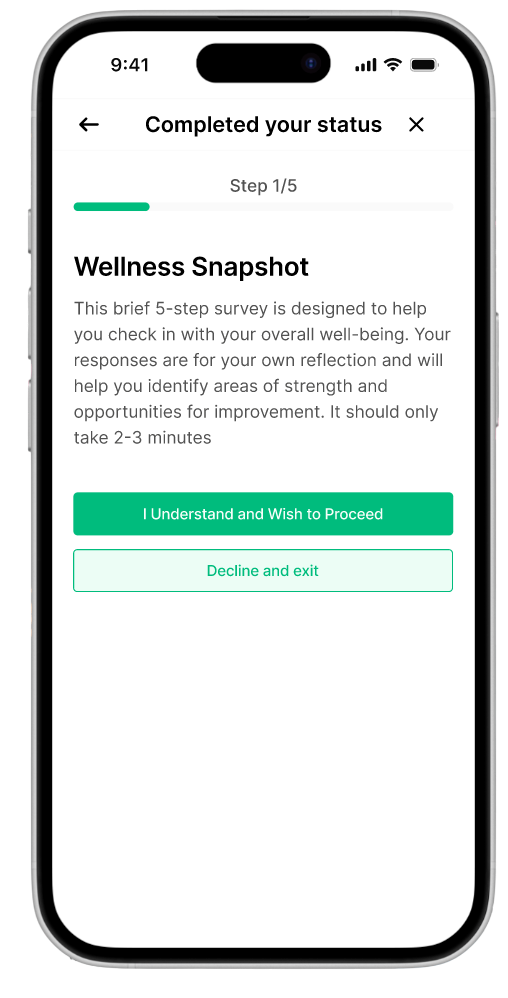
\includegraphics[width=\linewidth]{Images/Survey/step1.png}
        % Nếu CHƯA có ảnh thì comment dòng trên và mở dòng dưới:
        % \todobox{Splash Screen}
        \caption{Survey Step 1}
    \end{subfigure}
    \hfill
    \begin{subfigure}[b]{0.32\textwidth}
        \centering
        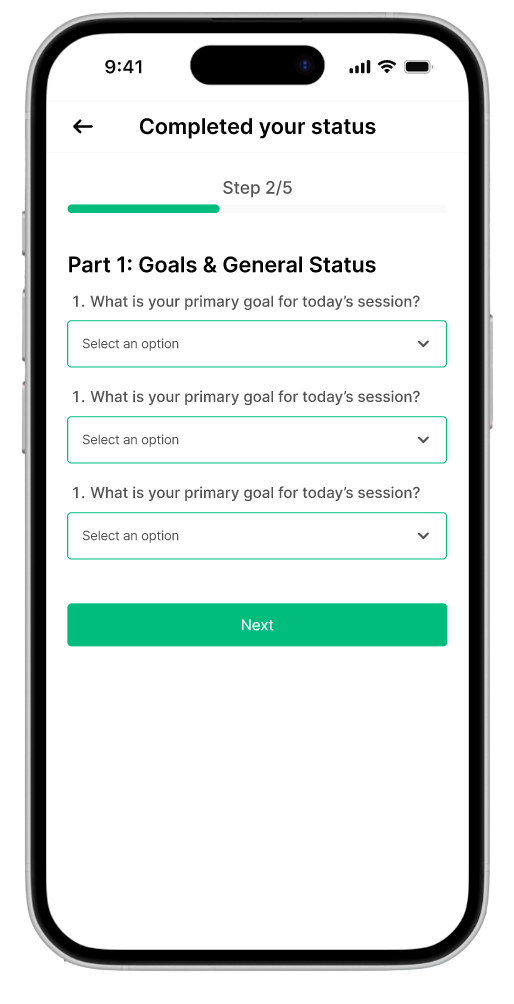
\includegraphics[width=\linewidth]{Images/Survey/step2.png}
        \caption{Survey Step 2}
    \end{subfigure}
    \hfill
    \begin{subfigure}[b]{0.32\textwidth}
        \centering
        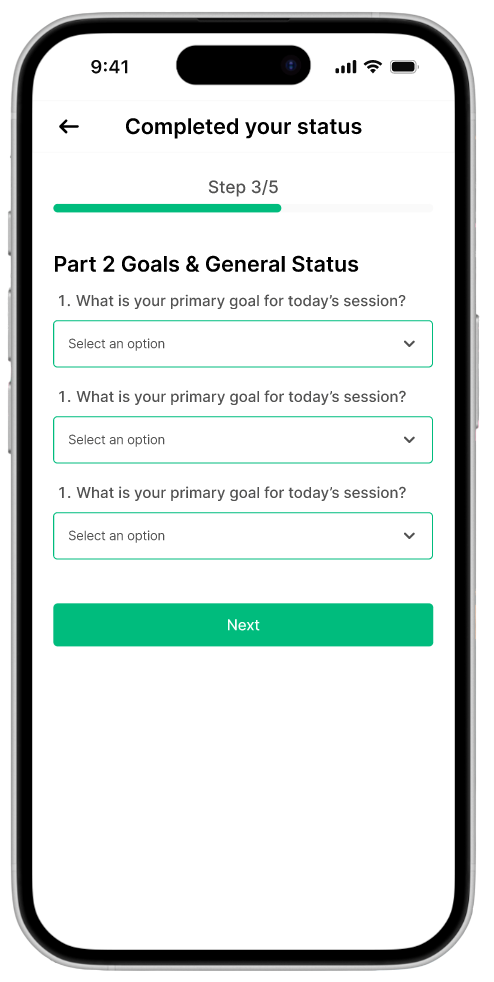
\includegraphics[width=\linewidth]{Images/Survey/step3.png}
        \caption{Survey Step 3}
    \end{subfigure}
    
    \vspace{1em} % Khoảng cách thoáng giữa 2 hàng
    
    % --- Hàng 2 ---
    \begin{subfigure}[b]{0.32\textwidth}
        \centering
        % Lưu ý: Bạn đang dùng lại ảnh signup_email.png, hãy check lại nếu cần
        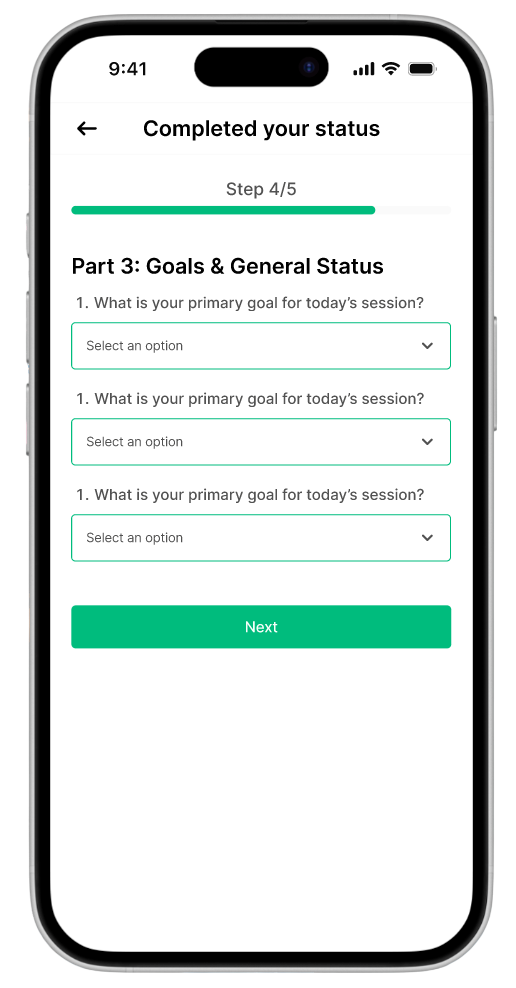
\includegraphics[width=\linewidth]{Images/Survey/step4.png}
        \caption{Survey Step 4}
    \end{subfigure}
    \hfill
    \begin{subfigure}[b]{0.32\textwidth}
        \centering
        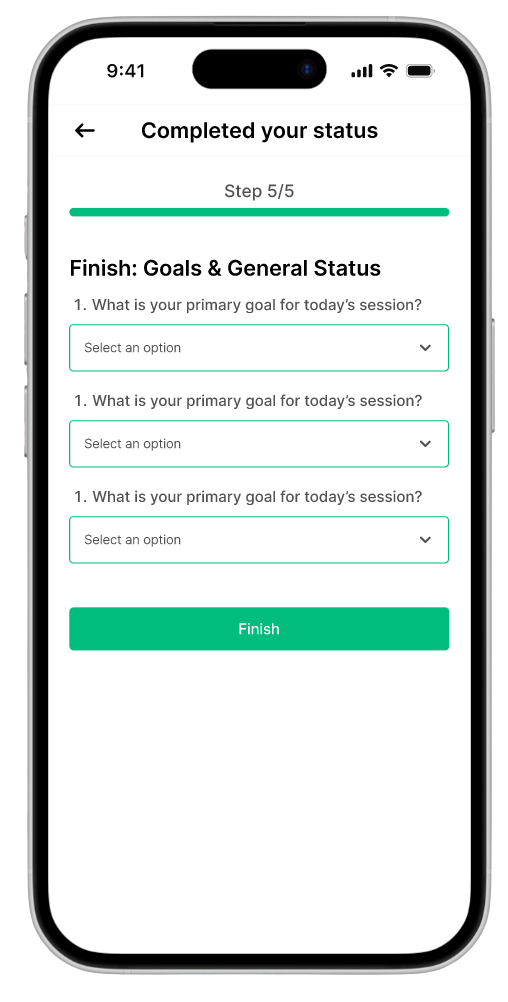
\includegraphics[width=\linewidth]{Images/Survey/step5.png}
        \caption{Survey Step 5}
    \end{subfigure}
    \hfill
    \begin{subfigure}[b]{0.32\textwidth}
     \centering
        
\includegraphics[width=\linewidth]{Images/blank_screen.png}
    \end{subfigure}
\end{figure}
\subsection{Main pages}

\begin{figure}[H]
    \centering
    
    % --- Hàng 1 ---
    \begin{subfigure}[b]{0.32\textwidth}
        \centering
        % Nếu có ảnh thì dùng dòng dưới:
        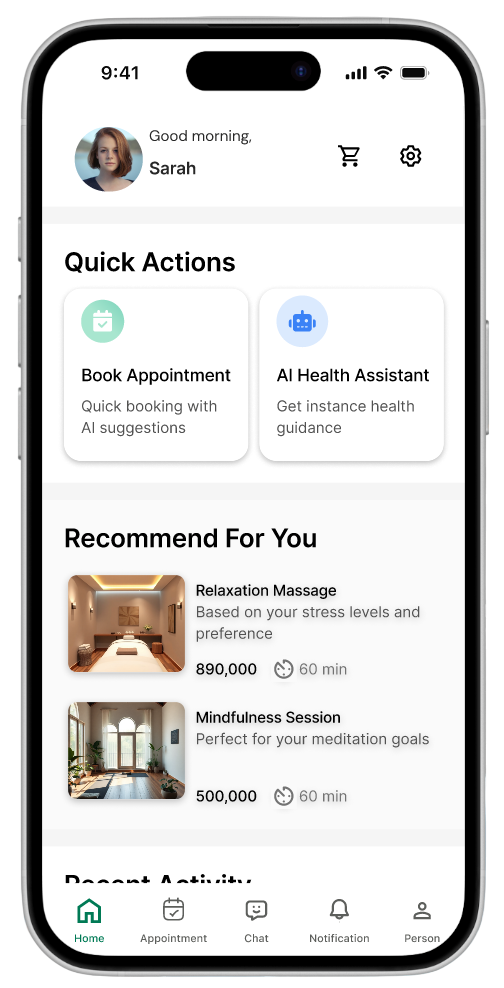
\includegraphics[width=\linewidth]{Images/Pages/home1.png}
        % Nếu CHƯA có ảnh thì comment dòng trên và mở dòng dưới:
        % \todobox{Splash Screen}
        \caption{Survey Step 1}
    \end{subfigure}
    \hfill
    \begin{subfigure}[b]{0.32\textwidth}
        \centering
        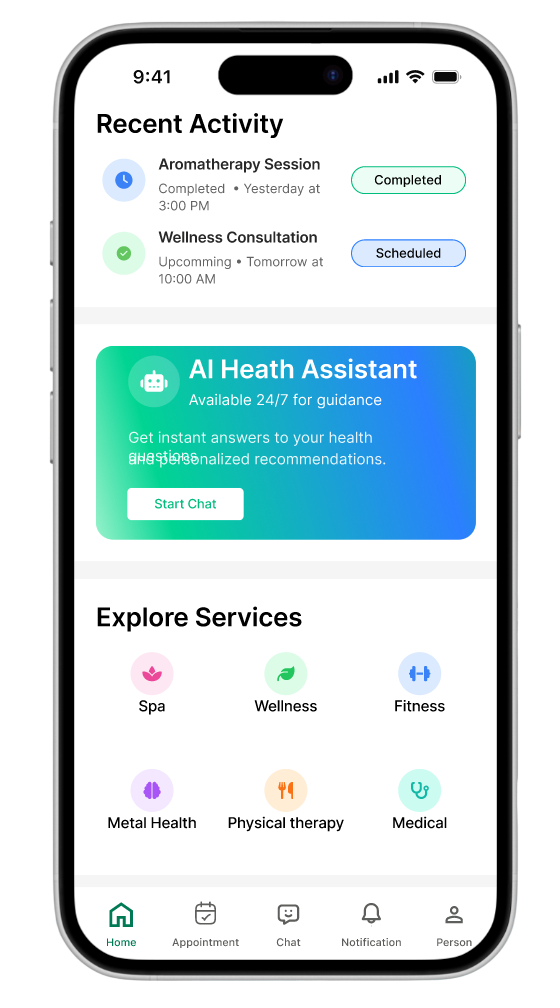
\includegraphics[width=\linewidth]{Images/Pages/home2.png}
        \caption{Survey Step 2}
    \end{subfigure}
    \hfill
    \begin{subfigure}[b]{0.32\textwidth}
        \centering
        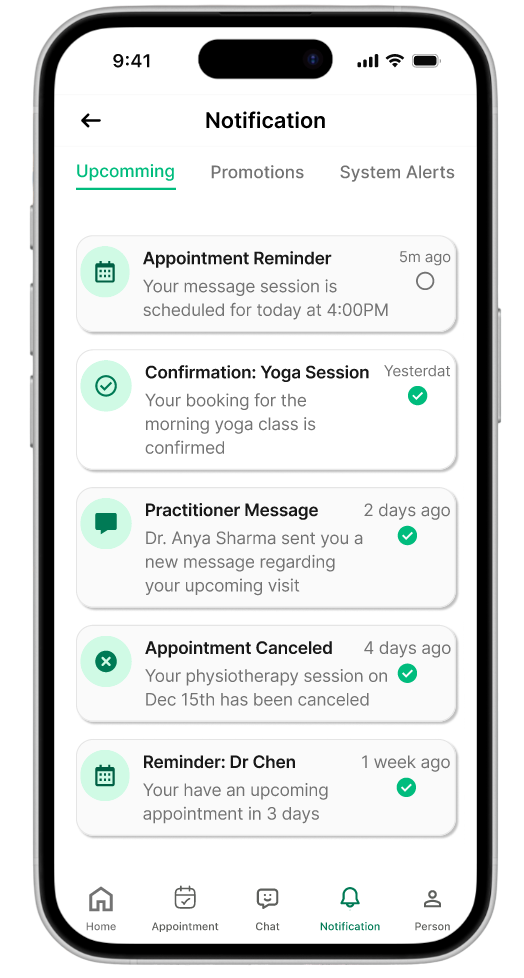
\includegraphics[width=\linewidth]{Images/Pages/noti.png}
        \caption{Survey Step 3}
    \end{subfigure}
    
    \vspace{1em} % Khoảng cách thoáng giữa 2 hàng
    
    % --- Hàng 2 ---                                                                                                                                
    \begin{subfigure}[b]{0.32\textwidth}
        \centering
        % Lưu ý: Bạn đang dùng lại ảnh signup_email.png, hãy check lại nếu cần
        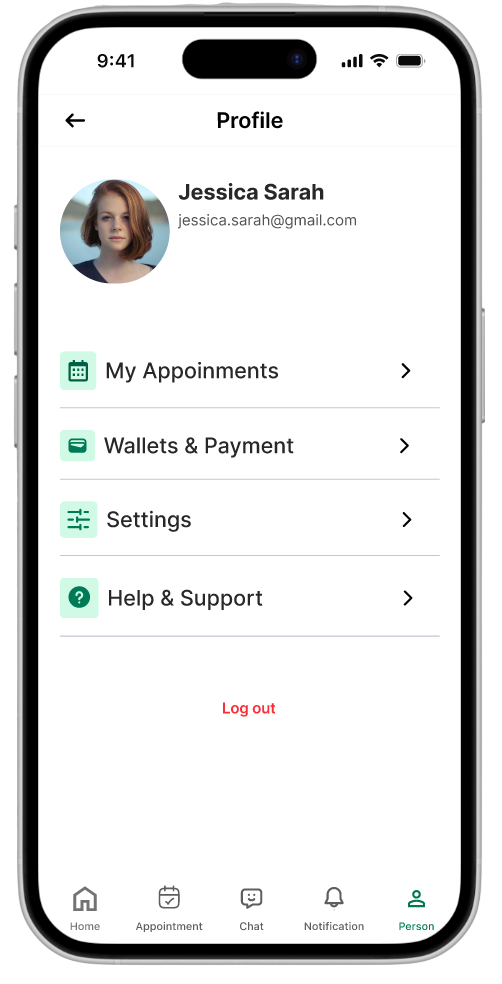
\includegraphics[width=\linewidth]{Images/Pages/profile.png}
        \caption{Survey Step 4}
    \end{subfigure}
    \hfill
    \begin{subfigure}[b]{0.32\textwidth}
        \centering
        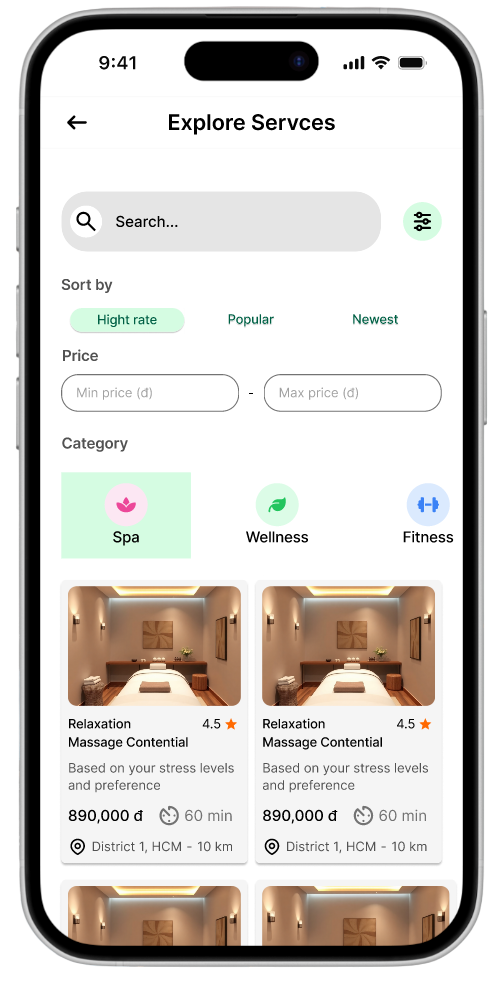
\includegraphics[width=\linewidth]{Images/Pages/services.png}
        \caption{Survey Step 5}
    \end{subfigure}
    \hfill
    \begin{subfigure}[b]{0.32\textwidth}
     \centering
        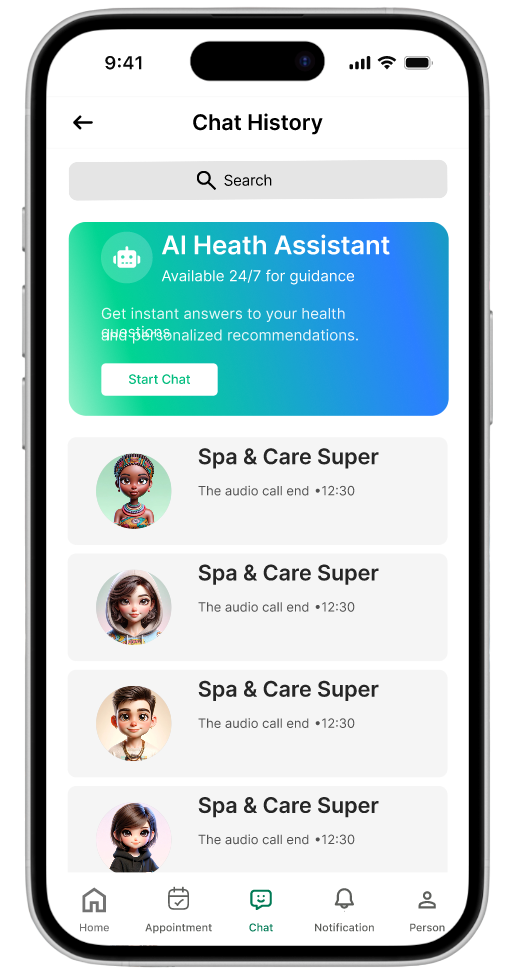
\includegraphics[width=\linewidth]{Images/Pages/chat.png}
         \caption{Chat}
    \end{subfigure}
\end{figure}

\section{Phần AI – Thiết kế \& Triển khai}
\subsection{Thu thập và tiền xử lý dữ liệu}
\begin{itemize}
    \item Lịch sử booking và hành vi người dùng
    \item Dữ liệu đánh giá \& phản hồi
    \item Chuẩn hóa và lưu trữ dữ liệu
\end{itemize}
\subsection{NLP Chatbot AI}

\subsubsection{Tổng quan}
Hệ thống NLP Chatbot AI được thiết kế nhằm xây dựng một trợ lý hội thoại thông minh có khả năng hiểu ngữ cảnh chuyên biệt theo từng miền (domain-specific) và luôn được cập nhật dữ liệu mới thông qua cơ chế \textbf{Retrieval-Augmented Generation (RAG)}.  
Mục tiêu chính là giúp mô hình vừa hiểu cách giao tiếp chuyên nghiệp (qua \textbf{fine-tuning}) vừa phản hồi theo thông tin thực tế mới nhất (qua \textbf{RAG}).

\subsubsection{Các bước chính}
\begin{itemize}
    \item \textbf{Fine-tuning:} Tạo nền tảng ngữ cảnh cho mô hình. Ví dụ: giúp mô hình hiểu rằng “BP” = “Blood Pressure” và biết cách phản hồi theo phong cách chuyên nghiệp.
    \item \textbf{RAG:} Cho phép mô hình luôn truy xuất dữ liệu mới, đảm bảo câu trả lời cập nhật và chính xác.
\end{itemize}

\subsubsection{Luồng dữ liệu chính (Data Flow)}

\noindent
\textbf{Luồng xử lý tổng thể:}

\begin{verbatim}
User hỏi
   |
   v
LangChain (PromptManager / Agent - định dạng lại prompt, chèn ngữ cảnh, lưu memory)
   |
   |--- RAG Retriever (FAISS / Chroma)
   |       |
   |       v
   |    Embedding Model (encode query)
   |       |
   |       v
   |    Vector DB (FAISS / Chroma)
   |       |
   |       v
   |    Context A (Kiến thức tĩnh)
   |
   |--- Database Tool (SQL / API)
           |
           v
        Context B (Dữ liệu động: đơn hàng, voucher, lịch, v.v.)
   |
   v
Context Builder
   - Gộp Context A + Context B + câu hỏi
   |
   v
LLM (LLaMa / Mistral)
   |
   v
LangChain Output Parser
   - Chuẩn hóa format
   |
   v
UI
\end{verbatim}
\subsubsection{Công nghệ và thành phần chính}
\begin{itemize}
    \item \textbf{PEFT (Parameter Efficient Fine-tuning):} Tổng hợp các phương pháp fine-tuning hiệu quả; trong đó \textbf{LoRA} là kỹ thuật phổ biến và hiệu quả nhất.
    \item \textbf{Hugging Face:} Nền tảng để tải model và thực hiện fine-tuning bằng LoRA.
    \item \textbf{LangChain:} Dùng để xây dựng pipeline hội thoại hoàn chỉnh:
    \begin{itemize}
        \item Tạo prompt động dựa trên câu hỏi người dùng.
        \item Gọi model (qua API hoặc local).
        \item Tích hợp công cụ: Database, RAG, truy xuất web.
        \item Quản lý hội thoại nhiều lượt (multi-turn).
        \item Tạo Agent reasoning tự động.
    \end{itemize}
\end{itemize}


\subsubsection{Pipeline RAG chi tiết}
Quy trình RAG bao gồm các bước sau:
\begin{enumerate}[label=\textbf{(\alph*)}, leftmargin=2cm, itemsep=4pt]
\item \textbf{Thu thập dữ liệu:} Bao gồm text, PDF, FAQ, transcript, blog, v.v.
\item \textbf{Tiền xử lý:} Làm sạch HTML, loại bỏ quảng cáo, chuẩn hoá tiếng Việt (có dấu), tách câu.
\item \textbf{Chunking:} Chia đoạn văn thành các phần nhỏ (200--500 tokens), thường sử dụng hàm \texttt{RecursiveCharacterTextSplitter} trong LangChain.
\item \textbf{Embedding:} Mã hoá từng đoạn bằng các mô hình embedding như \texttt{text-embedding-3-small} (OpenAI) hoặc \texttt{BAAI/bge-m3} (open source).
\item \textbf{Lưu trữ:} Lưu vector vào cơ sở dữ liệu tìm kiếm như \texttt{FAISS}, \texttt{Chroma} hoặc \texttt{Milvus}.
\item \textbf{Truy xuất:} Khi người dùng đặt câu hỏi, hệ thống sẽ mã hoá câu hỏi thành vector, tìm kiếm các đoạn có độ tương đồng cao nhất bằng \textbf{cosine similarity} hoặc thuật toán \textbf{MMR (Maximal Marginal Relevance)}.
\end{enumerate}


\subsubsection{Đánh giá hiệu năng (Evaluation)}
\begin{itemize}
    \item \textbf{Độ chính xác câu trả lời.}
    \item \textbf{Mức độ tự nhiên và tỷ lệ hallucination.}
    \item \textbf{Thời gian phản hồi (response time).}
\end{itemize}

\subsubsection{Quản lý phiên bản (Version Management)}
\begin{itemize}
    \item Tách riêng dữ liệu RAG (kiến thức cập nhật) và dữ liệu fine-tune (hiểu ngữ cảnh).  
    \item Ghi version rõ ràng: \texttt{rag\_v1}, \texttt{finetune\_v1}, \texttt{data\_2025\_10.json}.  
    \item Lưu trữ và quản lý bằng Git / DVC để dễ dàng rollback.  
\end{itemize}

\subsubsection{Cấu trúc dữ liệu huấn luyện (Fine-tuning)}
Chỉ áp dụng khi thực hiện fine-tuning, không cần cho RAG.

\noindent
\textbf{Trường hợp 1 — Câu hỏi đơn giản:}
\begin{verbatim}
{
 "instruction": "Khách hỏi: Tôi bị mụn ẩn thì nên chăm sóc thế nào?",
 "input": "",
 "output": "Bạn nên làm sạch sâu 2 lần mỗi ngày và dùng serum chứa BHA.
 Nếu mụn nhiều, nên chọn liệu trình Detox Skin tại spa."
}
\end{verbatim}

\noindent
\textbf{Trường hợp 2 — Câu hỏi có thông tin phụ (input):}
\begin{verbatim}
{
 "instruction": "Khách gửi thông tin da và muốn được tư vấn.",
 "input": "Da dầu, mụn cám, thường làm việc văn phòng, ít ra nắng.",
 "output": "Bạn nên chọn liệu trình kiểm soát dầu, tẩy da chết nhẹ 2 lần/tuần
 và đắp mặt nạ than hoạt tính để giảm bít tắc lỗ chân lông."
}
\end{verbatim}

\noindent

\subsubsection{So sánh mô hình}
\begin{center}
\renewcommand{\arraystretch}{1.3}
\begin{tabular}{|p{3cm}|p{6cm}|p{6cm}|}
\hline
\textbf{Model} & \textbf{Ưu điểm} & \textbf{Hạn chế} \\
\hline
\textbf{Mistral-7B} &
\begin{itemize}[leftmargin=*]
    \item Nhẹ, tốc độ suy luận nhanh.
    \item Mở nguồn, dễ triển khai và tích hợp.
    \item Cộng đồng hỗ trợ mạnh, có nhiều tài nguyên tinh chỉnh.
\end{itemize}
&
\begin{itemize}[leftmargin=*]
    \item Hiệu năng giảm khi xử lý context dài.
    \item Chưa tối ưu cho tiếng Việt (thiếu dữ liệu huấn luyện ngôn ngữ địa phương).
    \item Độ chính xác thấp hơn so với các mô hình lớn hơn.
\end{itemize}
\\
\hline
\textbf{LLaMA-3 (7B–13B)} &
\begin{itemize}[leftmargin=*]
    \item Hiệu năng cao trong tiếng Anh và đa ngôn ngữ chính.
    \item Tài liệu, quyền truy cập và công cụ hỗ trợ mạnh.
    \item Dễ fine-tune cho nhiều tác vụ khác nhau.
\end{itemize}
&
\begin{itemize}[leftmargin=*]
    \item Yêu cầu phần cứng mạnh (VRAM lớn, GPU nhiều).
    \item Cồng kềnh, khó triển khai trong môi trường hạn chế.
    \item Hạn chế trong tiếng Việt, dễ sinh lỗi ngữ nghĩa.
\end{itemize}
\\
\hline
\textbf{PhoGPT-4B-Chat} &
\begin{itemize}[leftmargin=*]
    \item Tối ưu cho tiếng Việt, phản hồi tự nhiên trong hội thoại.
    \item Nhẹ hơn các mô hình quốc tế, dễ deploy.
    \item Phù hợp ứng dụng dịch vụ công, chăm sóc khách hàng.
\end{itemize}
&
\begin{itemize}[leftmargin=*]
    \item Hiệu năng tiếng Anh chưa cao, đặc biệt trong ngữ cảnh chuyên sâu.
    \item Cộng đồng/tài liệu hỗ trợ còn hạn chế.
    \item Chưa ổn định khi xử lý context rất dài.
\end{itemize}
\\
\hline
\end{tabular}
\end{center}



\subsubsection{Định hướng và triển khai}
\begin{itemize}
    \item Sử dụng LangChain + RAG để tạo bản demo ổn định, kiểm tra độ chính xác.  
    \item Thu thập dữ liệu hội thoại thực tế theo domain.  
    \item Fine-tune bằng LLaMA + LoRA.  
    \item Tối ưu hóa pipeline cho inference và deployment.  
\end{itemize}



%%%%%%%%%%%%%%%%%%%%%%%%%%%

\subsection{Hệ thống gợi ý dịch vụ cá nhân hóa}

Hệ thống gợi ý dịch vụ cá nhân hoá được xây dựng nhằm cung cấp cho người dùng các đề xuất chính xác, phù hợp với nhu cầu sức khỏe và điều kiện cá nhân. Mục tiêu của hệ thống là xử lý nhiều loại dữ liệu khác nhau (textual, categorical, numerical), chuẩn hóa chúng về một không gian biểu diễn thống nhất, sau đó sử dụng mô hình tìm kiếm vector (FAISS) để truy xuất các dịch vụ tương tự nhất.

\subsubsection{Chiến lược trích xuất và chuẩn hóa đặc trưng (Feature Engineering)}

Để đảm bảo khả năng hiểu ngữ nghĩa và so khớp nhu cầu của người dùng với dịch vụ, hệ thống tiến hành tách riêng từng loại dữ liệu theo pipeline như sau:

\paragraph{Textual Features}
Các đặc trưng dạng văn bản mang tính mô tả ngữ nghĩa sâu. Chúng được embedding trực tiếp bằng mô hình ngôn ngữ (BERT hoặc các biến thể tối ưu hơn cho lĩnh vực y tế). Các trường dữ liệu bao gồm:
\begin{itemize}
    \item \textbf{Name / Title}: tên dịch vụ, sản phẩm.
    \item \textbf{Description / Details}: mô tả chi tiết, lợi ích, hướng dẫn sử dụng, quy trình thăm khám.
    \item \textbf{Category / Type}: phân loại dịch vụ (y tế, dinh dưỡng, luyện tập thể thao, tư vấn tâm lý, \ldots).
    \item \textbf{Tags / Keywords}: từ khóa đặc trưng như ``tim mạch'', ``yoga'', ``tư vấn online'', ``phục hồi chức năng'', \ldots
\end{itemize}

Các trường này sau khi embed bằng BERT sẽ thu được vector ngữ nghĩa có chiều cố định (thường từ 384 đến 768 chiều).

\paragraph{Categorical Features}
Các đặc trưng dạng phân loại được ánh xạ bằng One-hot Encoding hoặc Embedding học được. Các trường phổ biến:
\begin{itemize}
    \item \textbf{Region / Location}: khu vực cung cấp dịch vụ.
    \item \textbf{Provider Type}: loại nhà cung cấp (bác sĩ, bệnh viện, phòng khám, trung tâm dinh dưỡng, nền tảng online).
\end{itemize}

Sau Encoder, vector categorical được nối trực tiếp (concatenate) với vector embedding từ phần text.

\paragraph{Numerical / Scalar Features}
Các đặc trưng dạng số được chuẩn hóa về miền \([0, 1]\). Một số thuộc tính cần chuẩn hóa ngược nhằm phản ánh ưu tiên của người dùng:
\begin{itemize}
    \item \textbf{Rating}: điểm đánh giá dịch vụ (scale trực tiếp).
    \item \textbf{Cost}: chi phí dịch vụ. Giá trị này được chuẩn hóa rồi áp dụng công thức $1 - normalized\_value$ để giảm ưu tiên cho chi phí cao.
    \item \textbf{Popularity / User Count}: số lượng người đã dùng hoặc chọn dịch vụ.
    \item \textbf{Availability Score}: mức độ sẵn sàng (đặc biệt với các dịch vụ online có slot theo giờ).
\end{itemize}

Tất cả numeric features sau khi scale được ghép vào vector tổng.

\subsubsection{Xây dựng Query Vector}

Để đảm bảo hệ thống gợi ý phù hợp cho cả trang chủ và chatbot, pipeline query được thiết kế linh hoạt:

\paragraph{Query Trang Chủ (Home Recommender)}
Query được xây từ:
\begin{itemize}
    \item \textbf{User Profile}: lịch sử thói quen, hồ sơ sức khỏe.
    \item \textbf{Các dịch vụ đã chọn}: tăng mức độ cá nhân hóa.
    \item \textbf{Global Trend}: xu hướng sử dụng dịch vụ chung của toàn hệ thống.
\end{itemize}

\paragraph{Query Chatbot}
Người dùng nhập một câu tự nhiên, hệ thống sẽ:
\begin{enumerate}
    \item \textbf{Trích xuất thực thể (Extract Entity)} bằng NER hoặc Regex đã tinh chỉnh trên tập dữ liệu y tế nhỏ.
    \item \textbf{Phân loại thực thể}: Text / Categorical / Numerical.
    \item \textbf{Mã hóa (Encode)}: BERT cho text, One-hot/Embedding cho categorical, scaling cho numerical.
    \item \textbf{Ghép thành Query Vector}.
\end{enumerate}

\subsubsection{Pipeline tổng thể hệ thống gợi ý}

Quy trình hoàn chỉnh từ input người dùng đến kết quả truy xuất như sau:

\begin{enumerate}
    \item \textbf{Extract Entity}:
    \begin{itemize}
        \item Dùng NER hoặc Regex để tách các thực thể quan trọng.
    \end{itemize}

    \item \textbf{Phân loại thực thể theo loại dữ liệu}:
    \begin{itemize}
        \item Textual (ví dụ: triệu chứng, bệnh lý, mô tả nhu cầu).
        \item Categorical (provider type, khu vực).
        \item Numerical (chi phí, số lượng, rating).
    \end{itemize}

    \item \textbf{Encode từng loại đặc trưng}:
    \begin{itemize}
        \item Text → BERT embedding.
        \item Categorical → One-hot / Embedding.
        \item Numerical → Normalize.
    \end{itemize}

    \item \textbf{Concat}: tạo vector biểu diễn thống nhất.

    \item \textbf{FAISS Search}: tìm các dịch vụ có vector gần nhất trong không gian embedding.
\end{enumerate}

\subsubsection{Ví dụ minh hoạ pipeline}

\textbf{Query người dùng:} ``Tư vấn online về thoái hoá đốt sống cổ, giá 1 triệu''

\begin{itemize}
    \item \textbf{Extract Entity} (NER/Regex):
    \begin{itemize}
        \item ``online'' → Provider Type
        \item ``thoái hoá đốt sống cổ'' → Medical Condition (Textual)
        \item ``1 triệu'' → Cost (Numerical)
    \end{itemize}

    \item \textbf{Mapping / Classification}:
    \begin{itemize}
        \item Provider Type → Categorical
        \item Condition → Text
        \item Money → Numerical
    \end{itemize}

    \item \textbf{Encoding}:
    \begin{itemize}
        \item Text → BERT
        \item Categorical → One-hot
        \item Numerical → Normalize
    \end{itemize}

    \item \textbf{Concat} → Query Vector → FAISS Retrieval.
\end{itemize}

Hệ thống từ đó trả về các dịch vụ phù hợp nhất dựa trên tương đồng vector.





%%%%%%%%%%%%%%%%%%%%%%%%%%%%%%%%%%%%%%%%%
\subsection{Smart Notification System}
\begin{itemize}
    \item Gửi thông báo dựa trên hành vi người dùng
    \item Tối ưu thời điểm và nội dung thông báo
\end{itemize}
\subsection{Dashboard \& Business Analytics}
\begin{itemize}
    \item Các chỉ số đo lường hiệu quả AI
    \item Visualization \& KPI
\end{itemize}
\subsection{Thử nghiệm \& đánh giá mô hình AI}
\begin{itemize}
    \item Metrics: Accuracy, Precision, Recall, F1-score
    \item Case study gợi ý dịch vụ cho user thực tế
\end{itemize}
